\documentclass{report}
\usepackage[margin=1in, paperwidth=8.5in, paperheight=11in]{geometry}
%Math packages%
\usepackage{amsmath}
\usepackage{amssymb}
\usepackage{amsthm}
%Spacing%
\usepackage{setspace}
\onehalfspacing
%Lecture number%
\newcommand{\lectureNum}{14}
%Variables - Date and Course%
\newcommand{\curDate}{February 3, 2017}
\newcommand{\course}{MATH 239}
\newcommand{\instructor}{Luke Postle}
%Defining the example tag%
%\theoremstyle{definition}%
\newtheorem{ex}{Example}[section]
%Setting counter given the lecture number%
\setcounter{chapter}{\lectureNum{}}
%Package for drawing graphs%
\usepackage{tikz}
\usepackage{verbatim}
\usetikzlibrary{arrows}

\begin{document}
%Note title%
\begin{center}
\begin{Large}
\textsc{\course{} | Lecture \lectureNum{}}
\end{Large}
\end{center} 
\noindent \textit{Bartosz Antczak} \hfill
\textit{Instructor: \instructor{}} \hfill
\textit{\curDate{}}
\rule{\textwidth}{0.4pt}

% Actual Notes%
\subsubsection{Review from Last Lecture}
A \textbf{face} is a connected region of $\mathbb{R}^2 - (E(G) \cup V(G))$. Two faces are \textit{adjacent} if they share an edge. The \textit{degree} of a face $f$, $\mathrm{deg} (f)$, is equal to the number of edges in the boundary of $f$, where bridges are counted twice.\\
We also covered \textbf{Euler's Formula}
$$V - E + F = 1 + \,(\mathrm{\# \, of \, components})$$
For a connected graph, the number of components is 1, and so
$$V - E + F = 2$$
\section{More on Faces}
\subsection{Theorem 1}
\begin{center}
\textit{If G is a planar graph with $V \geq 3$, then $E \leq 3V - 6$}
\end{center}
\subsubsection{Proof of Theorem 1}
If $f$ is a face of $G$, then $\mathrm{deg}(f) \geq 3$ unless the boundary of $f$ contains at most one edge, but then $G$ would contain at most one edge. This motivates two cases:
\begin{itemize}
\item \textbf{Case 1:} $\vert E(G)\vert \leq 1$. But then $E \leq 3 \leq 3V - 6$ since $V \geq 3$.
\item \textbf{Case 2:} $\vert E(G) \vert \geq 2$. From what we said above, $\mathrm{deg}(f) \geq 3$ for all $f$. By the handshaking lemma for faces, we have $$2E = \sum_f \mathrm{deg}(f) \geq \sum_f 3 = 3F$$ So $F \leq \frac{2}{3}E$. Now, by Euler's formula
$$V - E + F \geq 2 \quad \text{(because the number of components is at least 1)} $$
And by our previous calculation, this yields
$$V - E + \frac{2}{3}E = v - \frac{E}{3}$$
Combining, we have
$$V - \frac{E}{3} \geq 2 \implies E \leq 3V - 6 \quad \text{QED}$$ 
\end{itemize}
\subsection{Corollary 1}
\begin{center}
\textit{$K_5$ is not planar}
\end{center}
\subsubsection{Proof of Corollary 1}
$\vert E(K_5) \vert = 10$ and $\vert V(K_5) \vert = 5$. If $K_5$ is planar, then by Theorem 1, $E \leq 3V - 6$. But for $K_5$, $10 \leq (3\cdot 5) - 6 = 9$, which is a contradiction.
\subsubsection{Observation 1}
Theorem 1 is nice, but note it is true for $K_{3,3}$, which as mentioned a few lectures ago, $K_{3,3}$ is not planar. We'll need a different condition to show that $K_{3,3}$ is non-planar.
\subsection{Theorem 2}
\begin{center}
\textit{If G is a triangle-free planar graph with $V \geq 3$, then $E \leq 2V - 4$}
\end{center}
\subsubsection{Proof of Theorem 2}
Consider two cases:
\begin{itemize}
\item \textbf{Case 1:} $E \leq 1$. But then $E \leq 1 \leq 2 \leq 2V - 4$, since $V \geq 3$
\item \textbf{Case 2:} $E \geq 2$. So $\mathrm{deg}(3) \geq 3$ for all $f$. Since $G$ is triangle-free, $\mathrm{deg}(f) \geq 4$ for all $f$. So we have $$2E = \sum_f \mathrm{deg}(f) \geq 4F \implies \frac{E}{2} \geq F$$
Combining, we have
$$V - \frac{E}{2} \geq 2 \implies E \leq 2V - 4 \quad \text{QED}$$
\end{itemize}
\subsubsection{Observation 2}
Observe that the Petersen graph satisfies Theorem 2; however, it too is not planar. This means that the contrapositive of this theorem is \textbf{not} true (similarly for Theorem 1).\\
Today, we have examined some necessary conditions that graphs have to meet in order to be planar, but they're not sufficient, since some non-planar graphs satisfy these conditions too. In the next lecture, we'll examine an if-and-only-if condition for planar graphs.
\newpage

\section{Platonic Solids}
The Greeks liked polyhedron (3D objects), and they especially liked ones with symmetry, such as when all of the faces had the same size or vertices all had the same degree. Observe that polyhedron can be modelled by graphs, thus we can study these objects using Graph Theory. Additionally, every polyhedron is a plane graph.
\subsubsection{Definition | Platonic Solid}
A \textit{platonic solid} is a plane graph where every vertex has the same degree $d \geq 3$, and every face has the same degree $d^* \geq 3$
\subsubsection{Question 1}
\begin{center}
Which graphs are platonic solids?
\end{center}
\subsection{Theorem 3}
\begin{center}
\textit{There exist only five platonic solids: tetrahedron, cube, octahedron, icosahedron, and the dodecahedron}
\begin{figure}[ht]
\begin{center}
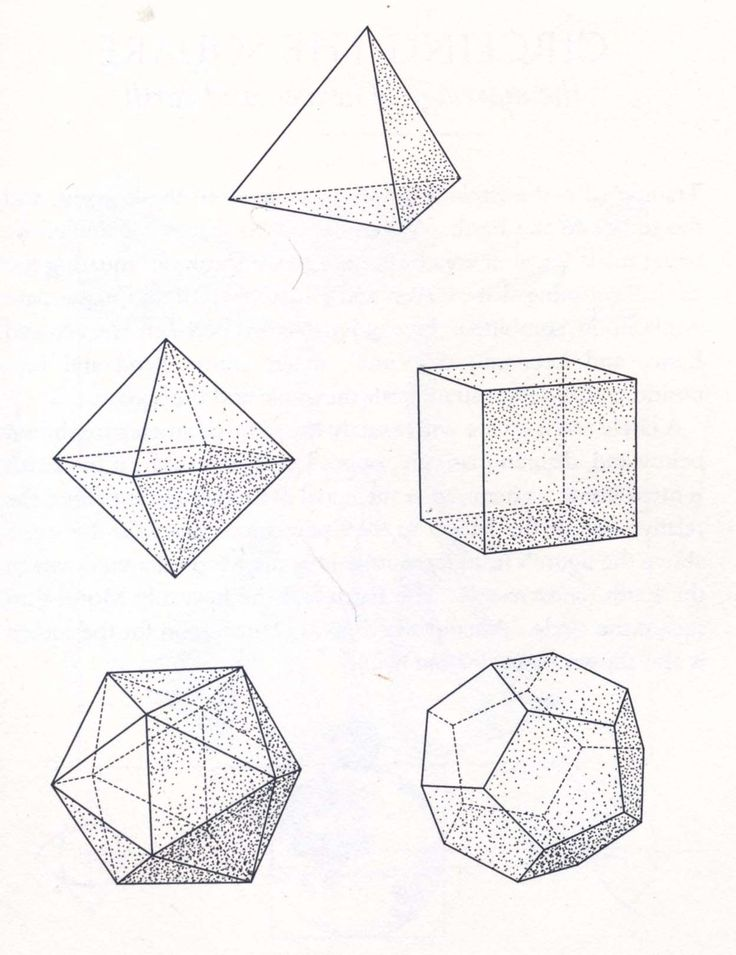
\includegraphics[scale=0.2]{platonic_solids.jpg}
\end{center}
\caption{Platonic Solids. Taken from Pinterest.}
\end{figure}

\end{center}
\subsection{Lemma 1}
\begin{center}
\textit{If G is a platonic solid, then $(d, d^*) \in \{(3, 3),(3,4),(3,5),(4,3),(5,3)\}$}
\end{center}
\subsubsection{Proof of Lemma 1}
By the handshaking lemma, $\displaystyle \sum_v \mathrm{deg}(v) = 2E = dV$. Additionally, by the handshaking lemma for faces, $\displaystyle \sum_f \mathrm{deg}(f) = 2E = d^*F$. So we have
$$V = \frac{2E}{d} \quad,\quad F = \frac{2E}{d^*}$$
But by Euler's formula
\begin{align*}
\frac{2E}{d} - E + \frac{2E}{d^*} &\geq 2 \\
\frac{2}{d} + \frac{2}{d^*} &\geq \frac{2}{E} + 1 && \text{(Divide by }E)
\end{align*}
Now observe four cases where this equation cannot be true:
\begin{itemize}
\item $d \geq 6, d^* \geq 3$ $$\frac{2}{E} + 1 \leq \frac{2}{6} + \frac{2}{3} = 1$$
This implies that $E = \infty$, a contradiction (when $d$ and $d^*$ get larger, the right-hand-side becomes less than 1, which also results in a contradiction).
\item $d=5, d^* \geq 4$ $$\frac{2}{E} + 1 \leq \frac{2}{5} + \frac{2}{4} < 1 \implies \frac{2}{E}  < 0$$
A contradiction. As $d$ and $d^*$ get larger, observe that $\frac{2}{E}$ is still less than zero, so nothing changes.
\item $d=4, d^* \geq 4$ $$\frac{2}{E} + 1 \leq \frac{2}{4} + \frac{2}{4} = 1$$
This implies that $E = \infty$, a contradiction (when $d$ and $d^*$ get larger, the right-hand-side becomes less than 1, which also results in a contradiction).
\item $d=3, d^* \geq 6$ $$\frac{2}{E} + 1 \leq \frac{2}{3} + \frac{2}{6} = 1$$
This implies that $E = \infty$, a contradiction (when $d$ and $d^*$ get larger, the right-hand-side becomes less than 1, which also results in a contradiction).
\end{itemize}
\begin{center}
\textit{The proof was finished here. More on this in the next lecture.}
\end{center}
%END%
\end{document}